\documentclass[12pt]{article}
\usepackage[top=1in, bottom=1in, left=1in, right=1in]{geometry}
\usepackage[justification=centering]{caption}
\usepackage{graphicx}
\usepackage{listings}
\usepackage{color}
\usepackage{indentfirst}
\usepackage{hyperref}
\usepackage{siunitx}
\usepackage{float}
\usepackage{amsmath}


\lstset{ %
	%language=C,                    % choose the language of the code
	basicstyle=\scriptsize,         % the size of the fonts that are used for the code
	backgroundcolor=\color{white},  % choose the background color. You must add \usepackage{color}
	showspaces=false,               % show spaces adding particular underscores
	showstringspaces=false,         % underline spaces within strings
	showtabs=false,                 % show tabs within strings adding particular underscores
	%frame=single,                  % adds a frame around the code
	tabsize=4,                      % sets default tabsize to 2 spaces
	captionpos=b,                   % sets the caption-position to bottom
	breaklines=false,               % sets automatic line breaking
	breakatwhitespace=false,        % sets if automatic breaks should only happen at whitespace
	escapeinside={\%*}{*)}          % if you want to add a comment within your code
}

\begin{document}
\title{Microprocessor Systems\\ Final Project: ANSI Target Game}
\author{Alvin Chia \and Nick Choi \and Samuel Deslandes \and Shanmugam Thiagarajan}
\date{12/13/16}
\maketitle
\pagebreak

\section{Introduction}
The overall goal of this project was to combine the content of several lab assignments in order to create an unique final product using the 8051. The idea that was pursued was an ANSI target game which utilized a keypad, a LCD display and an analog joystick module, and utilizes topics such as ANSI escape sequences, ADC conversions, timers, and interrupts. 

To begin, a menu screen needed to be created in order to give the user options to select before starting their game. Ultimately, the user would be given four options on the menu that represented the difficulty levels for the game. The number of targets and maximum time allowed on the level would be adjusted depending on which option was selected. The selections would be made using the keypad. Also displayed is a brief ``How to play'' statement. The player uses the joystick to move the cursor around on the screen, and presses the joystick to ``shoot'' the targets. 

Once the difficulty has been chosen, the game starts. Targets will be randomly drawn on the terminal display with a bullseye at the center of the target. Hitting the bullseye is worth 100 points, while any other zone on the target is worth only 10 points. Once all of the targets have been drawn, the timer begins to count down on the LCD display. The score is also displayed on the LCD screen and is updated whenever the user hits a new target. 

If the user completes the game before time runs out, they will be brought to a victory screen and will have the option to press the `\#' key in order to select a new difficulty. In the case that the user has only 5 seconds left, a buzzer will sound to alert the user of the remaining time. If the player fails to hit all of the targets in time, they will be brought to a game over screen, but will still have the option to press `\#' to return to the main menu and keep playing. 

\section{Methods}
\subsection{Software}
The program for this project was organized into several functions. The `main()' function handles initializations and repeatedly calls the `playGame()' function on an infinite loop. `playGame()' handles the main game play operations such as the main menu, moving the cursor, keeping track of time and score and displaying them on the LCD screen, and checking win and lose game states. Other functions such as `drawTarget()', `checkTarget()', and `eraseTarget()' handle the display and hit detection aspects of targets. 

\subsubsection{Main() and Configurations}
`Main()' begins by disabling the watchdog timer and calling the various initialization functions. In `PORT\_INIT()' the crossbar is configured such that UART0 is enabled in the `XBR0' SFR, /INT0 and /INT1 are routed to port pins in `XBR1', and in 'XBR2' the crossbar is enabled with weak pull-up. Next global interrupts and external interrupt 1 is enabled using the bit addressable keywords `EA' and `EX1', respectively. /INT1 associated with the button on the joystick is also set to be triggered on falling edge by setting `IT1` to 1. Lastly the ports are configured. P0.0 and P2.0 are set for push-pull operation for use by TX and a buzzer respectively. Port3 is used by the keypad, and is configured such that its high nibble in push-pull mode with digital LO output, and its low nibble is in open-drain mode with high impedance. 

`SYSCLK\_INIT()' initializes the system clock to use just the external oscillator with a frequency of 11.0592\si{Mhz}. In `UART0\_INIT()' Timer1 is used to generate a baud rate 115200. To accomplish this Timer1 is configured using the `TMOD' SFR to be an 8-bit counter with auto-reload. The auto-reload value for the required baud rate is \texttt{0xFA}. A reference reload values for each timer, SYSCLK, and desired baud rate can be found on page 295 of the C8051 manual[3]. The UART itself is configured to be in mode 1 using the `SCON0' SFR. In 'ADC0\_INIT()', `ADC0CF' is set to \texttt{0xBF}, resulting in a gain term of $\frac{1}{2}$, and a SARclk of 230400\si{Hz}. The can be calculated as follows: 
\begin{gather*}
	ADC0SC=\frac{SYSCLK}{2\times SARclk}-1\\
	\textrm{where ADC0SC is bits 3--7 of ADC0CF}
\end{gather*}
The internal reference buffer and bias generator are enabled, producing a voltage of 2.4\si{V}, which is used as a reference for conversions. All inputs are also treated as single-ended inputs.

Finally, Timer0 is used to accurately count game time in measurements of a tenth of a second. It's configured as a 16-bit counter using SYSCLK/48 as a base. For an overflow of this timer to occur every tenth of a second, the timer must be set to start counting at \texttt{0xA600} on initialization as well as after every overflow. This can be calculated as follows:
\begin{gather*}
	\frac{1}{48}\times \frac{11059200 \si{counts}}{\si{1}{sec}}=\frac{X\si{counts}}{0.1\si{sec}}
\end{gather*}
Solving for $X$ gives $X=23040$. Since 23040 counts elapse in a tenth of a second, the timer must start counting from $2^{16}-23040=42496$. This corresponds to \texttt{0xA600} in hex. Since Timer0 is a 16-bit counter, this must be split between its high and low registers, with $\mathrm{TH0}=\texttt{0xA6}$ and $\mathrm{TL0}=\texttt{0x00}$.

\subsubsection{playGame()}
The `playGame()' function starts by initializing the cursor position variables `xPos' and `yPos' to 1 because indexing for the terminal starts at 1 rather than 0, then resets the terminals main parameters, clears the screen, and calls the `Menu()' function. The terminal can be controlled by the software via ANSI escape sequences. Table \ref{ANSI} in the Appendicies section below show the sequences used in this program and their functions. The `Menu()' function displays the four difficulty option available to the player (Easy, Medium, Hard, and GG) to the terminal, and awaits user input from the keypad. This is done using the `getkeychar()' function which continuously polls a flag variable set by the keypad vector /INT0 ISR and returns the character pressed by the user.

The previously mentioned /INT0 ISR is connected to the hardware on P0.2, and is triggered on a falling edge. Once /INT0 has been triggered, the ISR must decode the signals on port 3 to determine which key has been pressed. The ISR starts by temporarily disabling interrupts on /INT0, then sets the flag variable used in `getkeychar()'. The rows of the keypad are decoded first, but before this the lower nibble of P3 is stored in a variable for later use. Once this is done, the output pins on P3 (high nibble) is set to \texttt{0x8}, \texttt{0x4}, \texttt{0x2}, then \texttt{0x1}, corresponding to rows 1--4 on the keypad respectively. After each change a small delay is implemented and the input pins on P3 (low nibble) are evaluated to see if they equal \texttt{0xF}; if so, then that is the row that had been selected. Columns are decoded using the original value of the low nibble of P3 stored before the decoding process. In this value all of the bits with be 1's, except for one; the selected column corresponds with the location of this bit, which can be determined by evaluating it to \texttt{0x07}, \texttt{0x0B}, \texttt{0x0D}, and \texttt{0x0E}. Once the selected column has been identified, a character can be assigned to a global variable ``asciichar'', which is returned by `getkeyhar()'. Figure \ref{KEY} in the appendices section can be used as a reference for which row and column intersection corresponds to which character. Once ''asciichar`` has been assigned P3 is reset to \texttt{0x0F}, and after another pause /INT0 is re-enabled and the program returns from the ISR. Once the user input is returned, a switch/case block is used to select the appropriate level. Which difficulty is selected dictates how much time the player has, as well as how many targets will be drawn to the screen. The table below shows the parameters for each difficulty. \\
\begin{table}[h]
	\centering
	\begin{tabular}{|l|l|l|}
		\hline
		Difficulty & Time (s) & \# of Targets \\ \hline
		Easy       & 60       & 5             \\ \hline
		Medium     & 45   	  & 7             \\ \hline
		Hard       & 30   	  & 9             \\ \hline
		GG         & 15   	  & 11            \\ \hline
	\end{tabular}
	\caption{Game level parameters}
	\label{difficulty}
\end{table}\\
Once these are set, the `drawTarget()' function is called, and the program returns to the `playGame()' routine. The details of `drawTarget()' will be discussed in the next section. 

Back in the `playGame()' function, the program then resets the cursor to its home position (1,1), starts Timer0, and enters an infinite loop. In this loop is where the game is played. First `readADC()' is called, which performs analog-to-digital conversions on the x and y inputs on the joystick, as well as from a potentiometer used to control the joystick sensitivity. ADC0 on the 8051 accepts up to 8 inputs, using a multiplexer to select a channel for conversion. The joystick y-axis is on channel 0 (AIN0.0), the x-axis on channel 1 (AIN0.1), and the potentiometer wiper on channel 3 (AIN0.2); the aforementioned multiplexer can be controlled via the `AMX0SL' SFR. An A-D conversion is initiated by setting `AD0BUSY'. The conversion process ends when the conversion interrupt flag goes digital LO, at which point the converted value can be read from the `ADC0' register. It is important to implement a small delay after changing channels on the multiplexer to allow the system to stabilize. 

Once these values have been read, the x and y-axis values are compared against threshold values, and the sensitivity value from the potentiometer is used to calculate a wait time for the while loop. If the x/y values exceed the thresholds, the cursor moves in the appropriate direction on the terminal, and the cursor position variables are updated. Checks are made to ensure that the cursor position does not exceed the playable range on the terminal\footnote{Playable region is defined by terminal row and column settings}. The cursor position is changed using ANSI escape sequences. The sensitivity value is mapped to wait times ranging from 655350--27035. This wait time is the time between each ``frame'' of the game. As such, the longer the wait time, the slower the cursor speed and the more control the player has over the cursor; conversely, the smaller the wait time the faster the cursor moves, allowing the player to reach more targets in a shorter span of time. The mapping from the converted sensitivity value to a wait time is as follows: 
\begin{displaymath}
	\mathrm{Wait\_time}=-11\times \mathrm{sensitivity}+65535
\end{displaymath}
This wait time has no affect on the time keeping mechanism of the game, as this is done via interrupts. Every tenth of a second the Timer0 ISR is triggered and a counter variable representing the number of elapsed tenths of seconds is incremented. In the `playGame()' infinite loop this counter is evaluated and if it equals 10, it is reset and the time variable set based on difficulty is decremented. 

In order to give user feedback, the amount of time remaining as well as the player's score is displayed on the first and second lines on the LCD respectively. All LCD functions can be found in the ``LCD.c'' file as well as its header file, which should be included. Before anything is printed to the LCD, the screen is cleared using `lcd\_clear()'. Next, using `sprintf()', the first line is prepared to be sent to the LCD. Calling `lcd\_goto(0)' moves the cursor to the top left corner and `lcd\_puts()' will print the prepared ``string'' to the LCD. The same is done for the second line, using `lcd\_goto(\texttt{0x40})' to move the cursor into the correct position. When there is 5 seconds remaining, output pin P2.0 is set to digital HI, which activates a buzzer; at 4 seconds remaining P2.0 is set back to digital LO and the buzzer turns off. 

The other remaining tasks of the `playGame()' are checking end game conditions. If the player has hit all of the targets, `WinScreen()' is called and a victory screen is printed to the terminal. If the player fails to eliminate all of the targets before time runs out, the `LoseScreen()' function is called an a game over screen is displayed. In both cases, the program breaks out of the infinite loop within `playGame()', and using `getkeychar()', the program will wait until the player presses the `\#' character on the keypad, at which point the function returns to `main()', where 'playGame()' is called yet again. 

\subsubsection{Target handling}
The functions `drawTarget()', `checkTarget()', and `eraseTarget()' deal with the displaying of the targets onto the terminal as well as hit detection. As mentioned before, `drawTarget()' is called after a difficulty selection is made within the `Menu()' function. This function draws the required number of target onto the terminal at random positions. The function starts by clearing the terminal, then for each target to be drawn, a random row and column is chosen using the `rand()' function. These coordinates represent the center of the target and are added to arrays which store the coordinates of the targets. To draw the targets, the program moves the cursor to the position one above and to the left of the center, and prints three blocks\footnote{U+2588, 219 on the extended ASCII table, cannot be displayed in \LaTeX} in white. In a similar manner 3 blocks are printed on the two rows below the first, creating a 3x3 box of block characters. The cursor is the moved to the center of the box and a red ``bullseye'' block is printed. 

When generating random locations for the center of targets, certain precautions are made to ensure that the entire target can be displayed, and that no two targets overlap. For the first case, random numbers are generated within the range from 2---($\#COLS-2$) for the columns, and 2---($\#ROWS-2$) for the rows, where \#ROWS and \#COLS represent the number of rows and columns the terminal displays. This is done using modular arithmetic using $row = rand()\%(\#ROWS-2)+2$ and $col = rand()\%(\#COLS-2)+2$. To ensure that no overlap between targets, each time a random position is generated, the program check this position against the positions of all the previously drawn targets and makes sure that the 3x3 boxes to be drawn are not in range of each other. 

The button the on joystick is connected to /INT1 on the 8051; as such when the button is pressed the associated `stickPress()' ISR function is called. This ISR calls the `checkTarget()' hit detection function, passing the current position of the cursor as its arguments. This function iterates through the arrays of target center positions and compares then to the passed in position. If passed in position is exactly the location of a target center, then the player is awarded 100 points to their score, and if it is one adjacent position away from the center, the player has hit the peripheral region of the target and the player is awarded 10 points. Once a hit has been detected the function stops iterating through the arrays of target positions, saves the cursors position, calls the `eraseTarget()' function passing in the center position of the target that was hit, restores the previously saved cursor position, decrements the variable storing the number of targets on the screen, and changes the values of the center position of the hit target both to 200. This is done to ensure that the player cannot hit the same target again, as 200 is outside the playable range.   

The `eraseTarget()' function performs identically to the 3x3 box drawing portion of the `drawTarget()' function. It moves the cursor to the positions one above and to the left of the passed in position, one to the left, and one below and to the left, printing three space characters at each position essentially overwriting the block characters with whitespace.
\subsection{Hardware}
\subsubsection{Joystick, Potentiometer, and Buzzer}
The analog joystick module used has 5 pins: 5\si{V}, V\_x, V\_y, SCL, and GND. The V\_x and V\_y pins output an analog voltage corresponding to how far in either direction the joystick is pushed. At its center position both pins output 2.5\si{V}; as the joystick is move up or to the right the output voltage increases to 5V, and decreases to 0V when moved in the opposite directions. These two pins were connected to AIN0.1 and AIN0.0 on the 8051, respectively. The SCL pin is connected to the button on the joystick; when pressed this pin outputs 0\si{V}. This is connected to /INT1 on the 8051 on P0.3. This corresponds to pin 19 on the 60-pin bus. 

A 10k\si{\ohm} potentiometer was also used as an analog voltage input source to the 8051. The positive terminal was connected to 5\si{V}, the negative to ground, and the wiper to AIN0.2 on the 8051, located on pin 49 on the 60-pin bus. 

A buzzer was also wired with the positive terminal connected to P2.0 of the 8051, and the negative terminal to ground. P2.0 corresponds to pin 29 on the 60-pin bus. 

Schematics for these components can be found in Figure \ref{others} in the appendices section below. 

\subsubsection{ADC}
This project called for use of the ADC on the 8051. Rather than using the pins on the 60pin bus for AIN0.0 and AIN0.1, the Analog I/O terminal block (J20) was used. A schematic for this can be viewed in Figure \ref{board layout} the appendicies section below. The internal 2.4\si{V} reference generator was used for VREF0. The output of the x and y-axes of the joystick were connected to AIN0.1 and AIN0.0 respectively. The sensitivity potentiometer output was connected to AIN0.2. AGND was connected to a common ground on the board. 

\subsubsection{LCD and Keypad}
In this project a LCD screen was wired to the 8051. A schematic for this can be viewed in Figure \ref{LCD} in the appendices section below. The LCD module used for this project has 14 pins.
Pins 1 and 2 are connections to ground and power, respectively. Pin 3 controls the screen contrast, which can be controlled using a potentiometer which comes as a part of the module. Pins 4, 5, and 6 are the register select, read/write select, and enable control signals, which were connected to P7.0--P7.2 on the 8051. Since port 7 was left in open-drain mode, a 10k\si{ohm} pull-up resistor was placed between P7.2 and power. Pins 7 to 14 are data pins, which were connected to all of port 6 on the 8051. Port 6 should be configured as open-drain with high-impedance on every pin. This does not have to be done explicitly in the code because this can be accomplished using the associated SFRs' default values.

A keypad was also interfaced to the 8051 for this project. A schematic can be viewed in Figure \ref{KEY} in the appendices section below. The keypad requires 8 wires, 4 for the columns and 4 for the rows, each of which are connected to port 3 on the 8051. The columns are connected to the lower nibble of port 3 (P3.0--P3.3) which is configured as open-drain for input. These wires are held high using a 3.3\si{V} and 10k\si{\ohm} pull-up resistors, and are also used as inputs to a four input and gate. The output of this gate is used as the /INT0 interrupt source and is connected to P0.2, corresponding to pin 20 on the 60-pin bus. The rows are connected to the high nibble of port 3 (P3.4--P3.7), which is configured as push-pull for output. These wires are held low by the software. 

\section{Results}
All of the intended features were successfully implemented. Starting from the main menu screen, the keypad accurately allowed for the user to select a difficulty and for each difficulty the correct number of targets were drawn and the correct amount of time was allotted. No overlap in targets or targets cropped by the edge of the terminal was observed. During game play when the joystick was moved the cursor moved accordingly, and a noticeable difference in cursor speed was observed when the sensitivity potentiometer was turned. Time was accurately being kept track of and displayed on the LCD screen along with the score which was promptly updated with the correct value when the player hit the target. As planned for, 100 points were awarded for hitting the bullseye, and 10 for hitting the outer tier. If the player pressed the joystick while not on a target, there was no change in score, even if there was previously a target drawn in that location. When there was 5 seconds remaining the buzzer turned on, and a second later turned off. Lastly, if the player ran out of the the game over screen appeared, and if the player hit all of the targets the victory screen was displayed. Pressing the `\#' key on the keypad on either of these screens successfully allowed the user to return to the main menu.

\section{Conclusion}
The results of our project matched the initial goals and expectations for the game. There are however additional features and improvements that can be made to the game. If given more time, a leaderboard feature could be added which would keep track of the highest scores obtained. Currently, the project uses most of the internal RAM available on the 8051 so additional RAM chips or the segment of xram addressed by ``xdata'' keyword would have to be utilized to properly store all of the game variables.


\section{Appendices}
\subsection{Code}
\lstinputlisting{main.c}
\subsection{Schematics}
\begin{figure}[H]
	\centering
	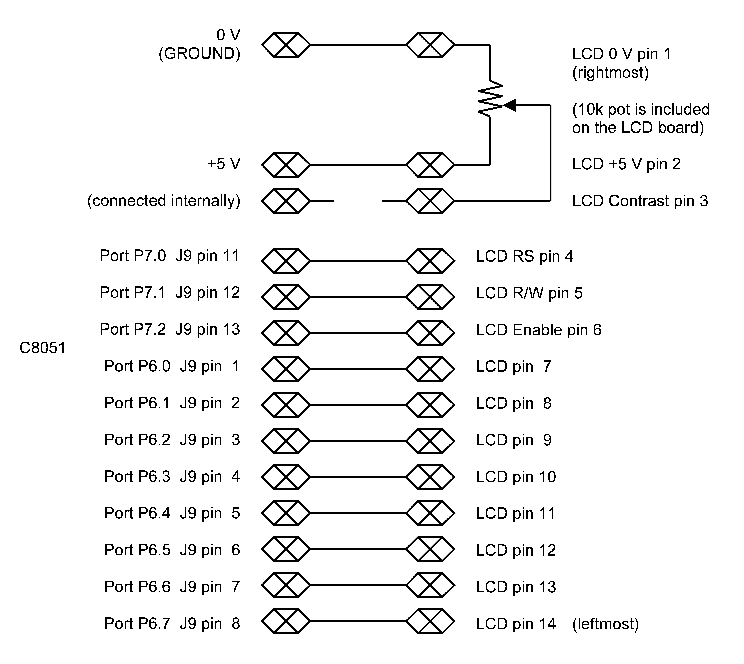
\includegraphics[width=\textwidth]{lcd_schematic.PNG}
	\caption[]{Circuit schematic for LCD[2]}
	\label{LCD}
\end{figure}
\begin{figure}[H]
	\centering
	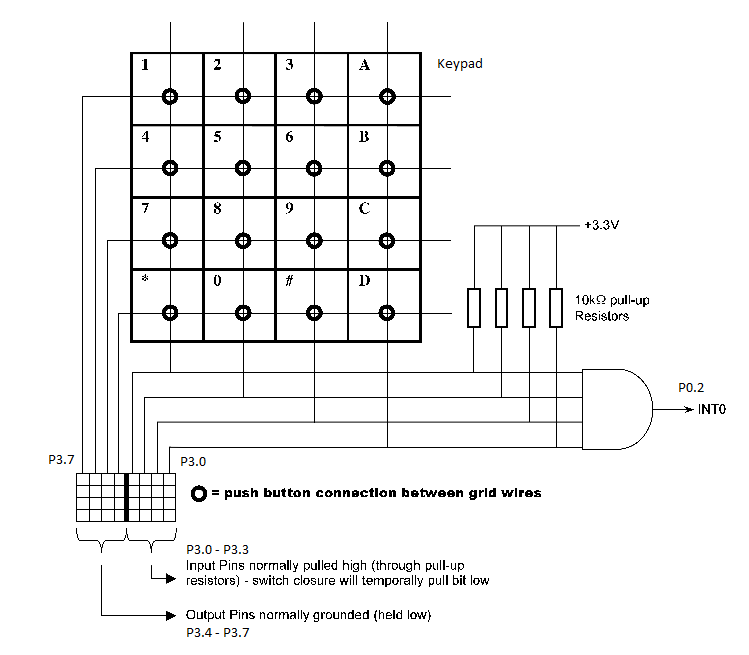
\includegraphics[width=\textwidth]{keypad_schematic.png}
	\caption[]{Circuit schematic for keypad[1]}
	\label{KEY}
\end{figure}
\begin{figure}[H]
	\centering
	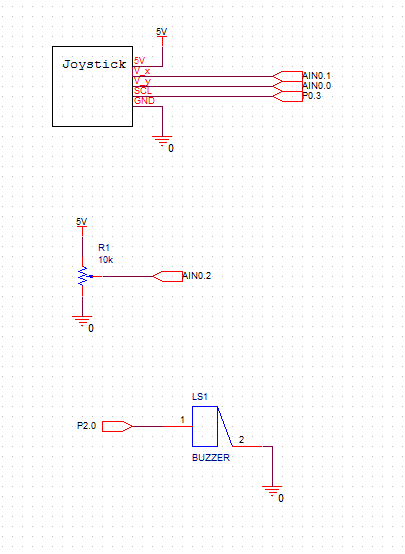
\includegraphics{OtherParts.PNG}
	\caption[]{Schematic for joystick, potentiometer, and buzzer connection}
	\label{others}
\end{figure}
\subsection{Analog I/O Terminal block}
\begin{figure}[H]
	\centering
	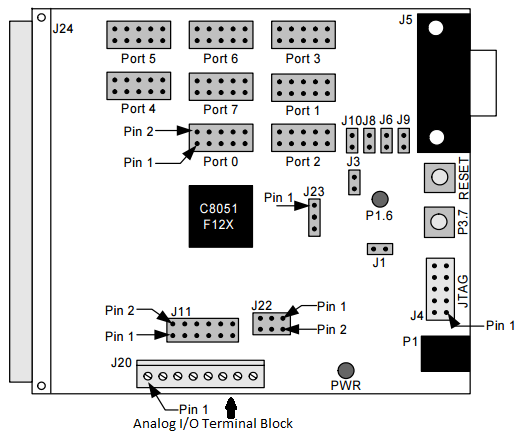
\includegraphics[]{board.PNG}
	\caption{C8051F120 Targer Board layout[1]}
	\label{board layout}
\end{figure} 
\begin{table}[h]
	\centering
	\begin{tabular}{|l|l|}
		\hline
		Pin\# & Description \\ \hline
		1 & CP0+\\ \hline
		2 & CP0-\\ \hline
		3 & DAC0\\ \hline
		4 & DAC1\\ \hline
		5 & AIN0.0\\ \hline
		6 & AIN0.1\\ \hline
		7 & VREF0\\ \hline
		8 & AGND (Analog Ground)\\ \hline
	\end{tabular}
	\caption{J20 Terminal Block reference table}
	\label{refTable}
\end{table}
\newpage
\subsubsection{ANSI Escape Sequence Table}
\begin{table}[h]
	\centering
	\begin{tabular}{|l|l|}
		\hline
		ANSI escape sequence & Function \\ \hline
		\textbackslash033[2J & Clear screen and return cursor to home \\ \hline
		\textbackslash033[1;33;43m & Set foreground color to yellow and background color to white, bright \\ \hline
		\textbackslash033[1;37m & Set foreground color to white, bright\\ \hline
		\textbackslash033[1;31m & Set foreground color to red, bright\\ \hline
		\textbackslash033[30m & Set foreground color to black, dim\\ \hline
		\textbackslash033[47m & Set background color to white, dim\\ \hline
		\textbackslash033[\{row\};\{col\}H & Move cursor position to (\{row\},\{col\})\\ \hline
		\textbackslash033[1A & Move cursor up one row \\ \hline
		\textbackslash033[1B & Move cursor down one row \\ \hline
		\textbackslash033[1C & Move cursor right one column \\ \hline
		\textbackslash033[1D & Move cursor left one column \\ \hline
		\textbackslash033[H & Return cursor to home position\\ \hline
		\textbackslash033[s & Save cursor position\\ \hline
		\textbackslash033[u & Restore cursor position\\ \hline
		
	\end{tabular}
	\caption{Quick reference table of ANSI escape sequences}
	\label{ANSI}
\end{table}
\section{References} 
\noindent
[1]``C8051F12x Development Kit User's Guide ,'' in RPI ECSE Department, Rev. 0.6,May 2005. [Online]. Available: \url{https://www.ecse.rpi.edu/courses/CStudio/Silabs/C8051F12x-DK.pdf}. Accessed: Dec. 12, 2016.\\
\newline\noindent
[2]``Interfacing a Hitachi HD44780 to a Silicon Laboratories C8051F120," in RPI ECSE Department, 2016. [Online]. Available: \url{http://www.rpi.edu/dept/ecse/mps/LCD_Screen-8051.pdf}. Accessed: Dec. 12, 2016.\\
\newline\noindent
[3]``C8051 Manual," in RPI ECSE Department, 1.4 ed., 2005. [Online]. Available: \url{https://www.ecse.rpi.edu/courses/CStudio/Silabs/C8051F12x-13x.pdf}. Accessed: Dec. 12, 2016.\\
\newline\noindent
[4]``MPS Lab 1," in RPI ECSE Department, 2016. [Online]. Available: \url{http://www.rpi.edu/dept/ecse/mps/MPS_Lab_Ex1-IDE_ANSI.pdf}. Accessed: Dec. 12, 2016.\\
\newline\noindent
[5]``Ascii Table - ASCII character codes and html, octal, hex and decimal chart conversion'', Asciitable.com, 2016. [Online]. Available: \url{http://www.asciitable.com/}. Accessed: Dec. 12, 2016.
	
	
\end{document}